\documentclass{article}
\usepackage[utf8]{inputenc}

\title{COP_290_ASSIGNMENT1}
\author{gupta.sauhard }
\date{9, March 2016}

\usepackage{graphicx}
\usepackage{caption}

\title{COP290: Complaint Management App}
\author{Prabhu Prasad Panda (2013ME10859) \\ 
Sauhard Gupta (2013ME10117) \\ 
Yash Kumar Bansal (2013ME10742) }

\begin{document}
\maketitle
   The \textbf{CMS} App is a mobile application of Complaint Management of IIT-Delhi. For User comfort the background is kept bright and the text fields are made large to ensure an easy viewing experience.Also the app guides the User through the various steps interactively and thus providing a user friendly interface.Lastly the application is easy to use.

\section{SCOPE}
\begin{itemize}
\item The Assignment aims to connect IIT Delhi community with Android Devices which includes:-
\begin{enumerate}
\item faculty
\item students 
\item staff/institute employees
\end{enumerate}
\item Using the app these end Users can submit their complaint/grievances to the concerned authorities.
\item Thus, the application allows for \textit{three} type of complaints:
\begin{enumerate}
\item \textbf{Individual complaint}: A student wants to complain about the electricity problem in his hostel room to an electrician
\item \textbf{ Hostel level complaint}: Hostel residents want to complain about
the bad quality of the mess food to their warden.
\item \textbf{ Institute level complaint }: Students across the institute want to protest against the LAN ban after 1 am.
\end{enumerate}
\item Lastly, we will  extend this assignment to web clients in addition to the Android clients, if time permits, since API's support exists.



\section{DATA STORAGE}
\begin{enumerate}
\item \textbf{Users Table:-}Every member of the complaint management system is stored in this table. It comprises of the following fields.
\begin{enumerate}
\item \textbf{*User ID} (which is a string field that stores the Kerberos ID of the user)
\item \textbf{*Password} (String Password Field)
\item \textbf{*Name} (String)
\item \textbf{Email ID} (other than the Kerberos mail id - String)
\item \textbf{Mobile}(Numeric-10 digits)
\item \textbf{*Address} (String)
\item \textbf{*Locality} (Enumerated Data Type includes hostels, apartments, outside IIT etc.) – The outside IIT people can’t raise complaints.
\item \textbf{Profile Pic} (Address)
\end{enumerate}
* - Compulsory Fields
Keys: User ID will act as primary key.
\item \textbf{Administrators Table:-} It stores the various administrative posts in the complaint management system and their corresponding hierarchies. The fields are:
\begin{enumerate}
\item \textbf{*Admin ID} (which stores the ID associated with a particular post.)
\item \textbf{*Admin Password} (Password for the admin account).
\item \textbf{*User ID} (which stores the User ID of the user from Users Table who is currently managing the post. It is set as null if there is a vacancy. Validation rule – It must exist in the Users Table.
\item \textbf{*Parent ID} (stores the Admin ID of the parent of this admin.)
\item \textbf{*Name} (name of the post)
\item \textbf{*Description} (details of the post)
\item \textbf{*isLeaf} (Boolean states whether it is a leaf-level admin or not)
 \end{enumerate}
 Any Group Level Complaint can be addressed only to a leaf-level admin who can approve the complaint and sent it to the solvers for solving or can forward it to a higher level admin. Each admin can conduct polls to get the general opinion.

The tree hierarchy must have the following root structure:


\end{enumerate}
                \begin{minipage}{\linewidth}
	        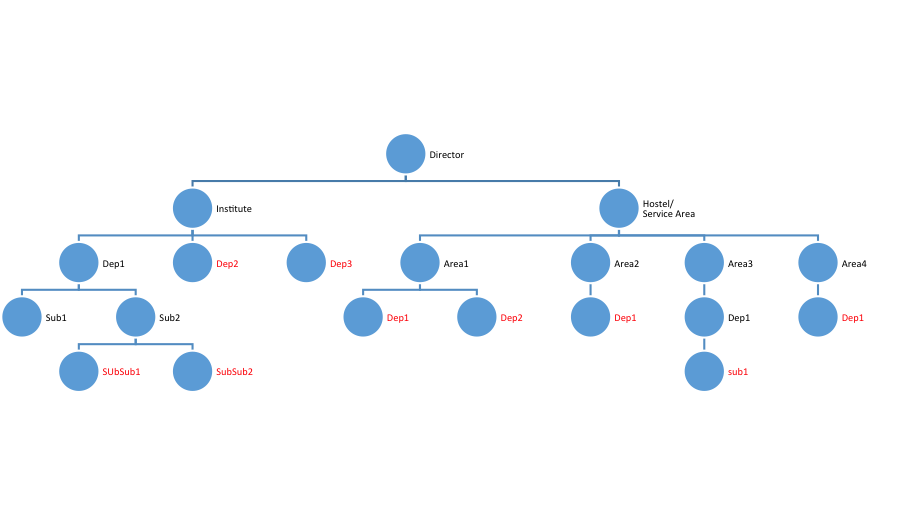
\includegraphics[scale=.9]{flowchart1.png}
	        \captionof{figure}{Hierarchy Tree}
            \end{minipage}
\item \textbf{Solvers Table:-}This table stores the various departments who solve the problem. Each department is managed by a single user. (Currently we are not considering any hierarchies in the solving department but there is scope for extension)
The fields are:

\begin{enumerate}
\item \textbf{*Solver ID}: Stores the ID associated with a solving department
\item \textbf{*Solver Password:} Password for the solver account.
\item \textbf{*User ID:} Stores the ID of the user managing the post
\item \textbf{*Department:} Name of the department
\item \textbf{*Description}: Details of the department

 \end{enumerate}
 
 \item \textbf{Individual Complaints Table:}It stores all the individual complaints (or the approved group complaints of which an individual complaint will be lodged from the approver). The fields are:


\begin{enumerate}
\item \textbf{*Complaint ID (key):} The ID of the complaint.
\item \textbf{*User ID:} The User ID of the person who lodged the complaint.
\item \textbf{*Solver ID:} The ID of the department to which the complaint is sent.}
\item \textbf{*Date:}  The date on which the complaint is lodged or approved
\item \textbf{*Status:} Status of the complaint
\item \textbf{*Title:} title of the complaint
\item \textbf{*Description:} details of the complaint
\item \textbf{Links:} Stores the links attached
\item \textbf{Images:} Stores the addresses of the images attached
\item \textbf{Approved/Discarded Date:} If it is approved or discarded, the date is stored here
 \end{enumerate}
            
 
 \item \textbf{Group Complaints Table:}It stores the group complaints. Once approved an individual complaint will be sent from the approver to the solvers’ department. The fields are:


\begin{enumerate}
\item \textbf{*Complaint ID (key):} The ID of the complaint.
\item \textbf{*User ID :} The ID of the user who lodged the complaint
\item \textbf{*Init Admin ID:} The ID of the leaf-level admin to which the complaint was initially addressed.
\item \textbf{*Cur Admin ID:} The ID of the Admin who is currently in charge of the complaint.
\item \textbf{*Date:} The date on which the complaint was lodged.
\item \textbf{*Transaction History:} It stores as text the history of transactions e.g., “forwarded by <admin1> to <admin 2> on <date><time>”.
\item \textbf{Title:} Title of the complaint
\item \textbf{Description:} Details of the complaint
\item \textbf{*Type:} Type of complaint (for ex: institute level or hostel level for area 1 etc.)
\item \textbf{*Status:} Status of the complaint
\item \textbf{Links:} Stores the links attached
\item \textbf{Images:} Stores the addresses of the images attached
\item \textbf{Poll Results:} Poll results stored as string in a specified format
\item \textbf{Approved/Discarded Date:} If it is approved or discarded, the date is stored here
 \end{enumerate}

\newline
\begin{minipage}{\linewidth}
	        
	        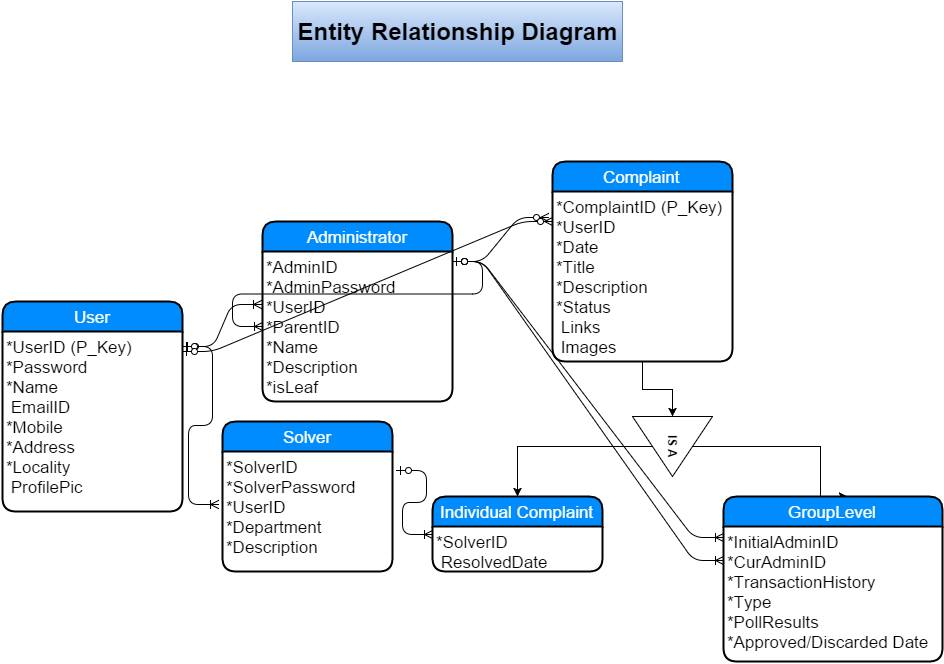
\includegraphics[scale=.4]{erd1}
	        \captionof{figure}{Entity Relationship Diagram}
            \end{minipage}
 
\section{APIs and EVENT FLOW}
\begin{enumerate}
\item \textbf{Login and Logout APIs:} We need to have APIs to enable login and logout. On logging in setCookie will be used to store the necessary cookie data in the device which includes encrypted information of the logged in user. This will be a session cookie and will be deleted as soon as the user logs out.
APIs:
\newline
-Logging in: domain/login/userid= userid &pswd= password 
\newline
-Logging out: domain/logout.json
\item A normal user must be able to see individual level complaints raised by him, hostel –level complaints for his/her hostel or area and institute level complaints.
\newline
APIs for the same:
\newline
\newline
\textbf{Individual level complaints: }From the cookie the User ID can be accessed and a query sent to he individual complaints table that all complaints with User ID same as the user should be sent as JSON.
\newline
API – domain/viewComplaints/Indilevel.json
\newline
Method- GET
\newline
\newline
\textbf{Hostel Level Complaints:} Similarly the group level complaints with type as the hostel level complaint from the hostel/area of the current user should be sent as JSON.
\newline
API – domain/viewComplaints/Arealevel.json
\newline
Method- GET
\newline

\textbf{Institute Level Complaints:} The group level complaints with type as Insititute level complaints should be displayed.
\newline
API – domain/viewComplaints/Instilevel.json
\newline
Method- GET

\item A normal user should be able to lodge and edit (sometimes) individual, hostel-level and institute level complaints. So accordingly 3 APIs will be provided for each of these and POST method will -be used to send the JSON information.
\newline
\textbf{-	Individual Level: }

\begin{minipage}{\linewidth}
	        \centering
	        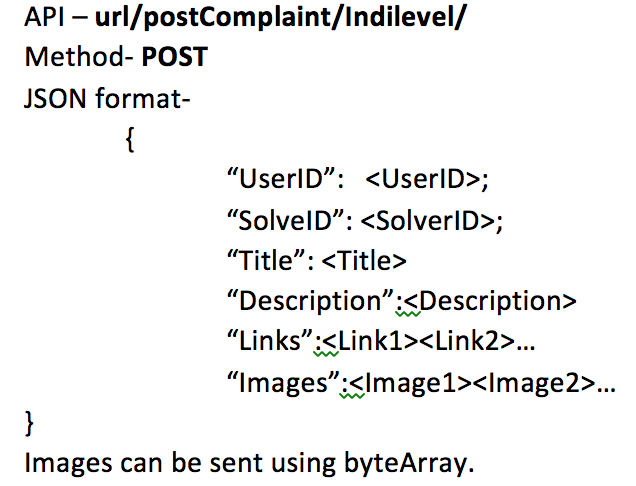
\includegraphics[scale=.6]{1.png}
	      
            \end{minipage}
\newline
\newline
\textbf{-	Hostel Level:}
\newline
\begin{minipage}{\linewidth}
	        \centering
	        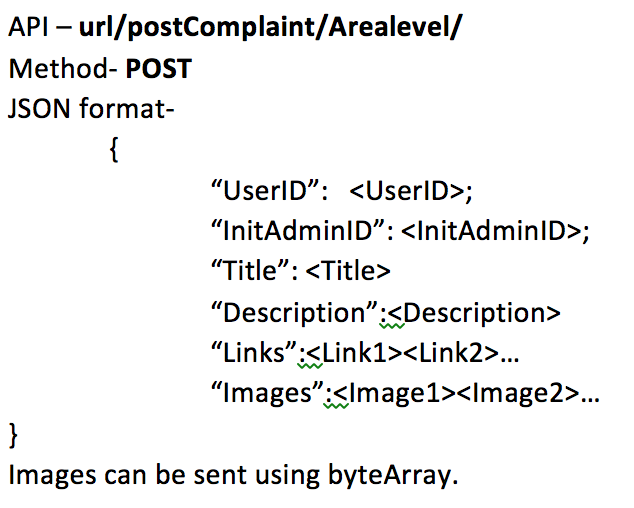
\includegraphics[scale=.6]{2.png}
	        
            \end{minipage}
\newline
\textbf{-	Institute Level:}
\newline
\begin{minipage}{\linewidth}
	        \centering
	        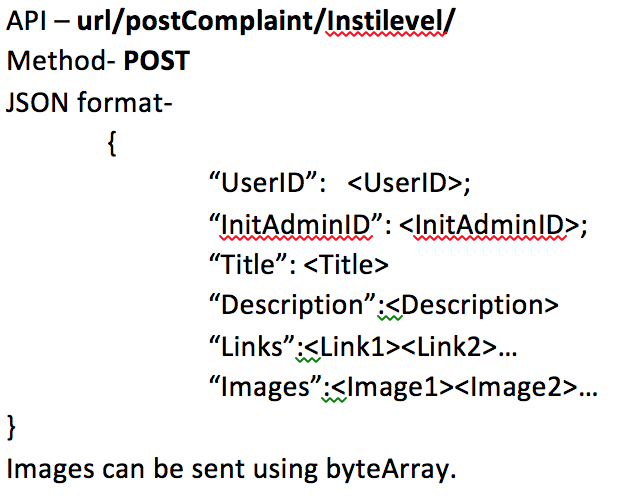
\includegraphics[scale=.6]{3.png}
            \end{minipage}
\item Administrators need to view the complaints addressed to them, the history of their works (complaints which they forwarded to a higher admin, discarded complaints, approved complaints etc.)  . The following describes the permissions for complaint viewing of administrators:
\newline
\begin{minipage}{\linewidth}
	        \centering
	        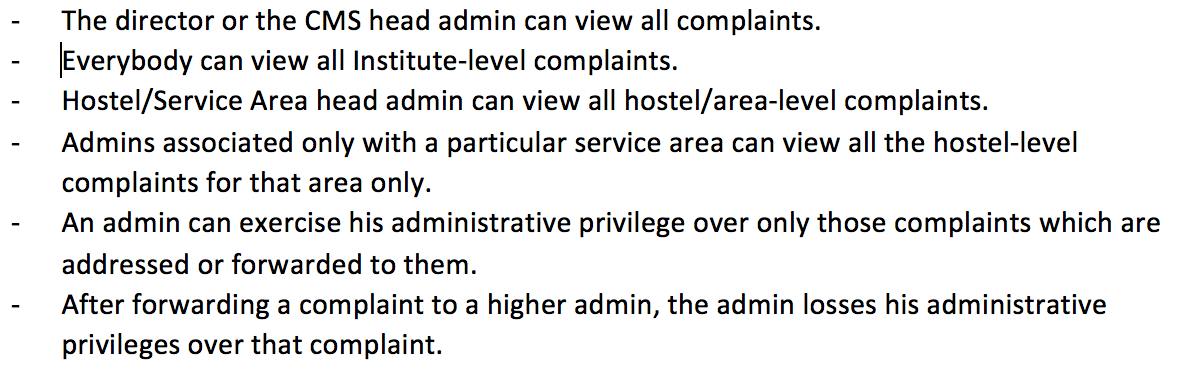
\includegraphics[scale=.5]{4.png}
            \end{minipage}
            \newline
            So according to the logged administrator (can be found from the cookie and will be sent along with the API), the APIs will be accessible. For example a hostel-level admin for a particular area will not have access to the hostel-level complaints of another area.
\newline
            
\begin{minipage}{\linewidth}
	        \centering
	        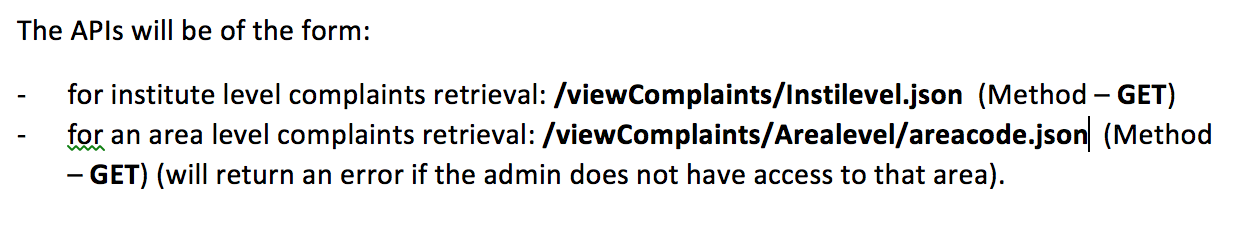
\includegraphics[scale=.5]{5.png}
            \end{minipage}
            \newline
            
\item \textbf{What can an Admin do?} He/she can approve, discard, start a poll and forward a complaint. So there has to be APIs for the same. All the fields except the polling will be discussed here. Polling will be discussed on the next point. 
\newline
            
\begin{minipage}{\linewidth}
	        
	        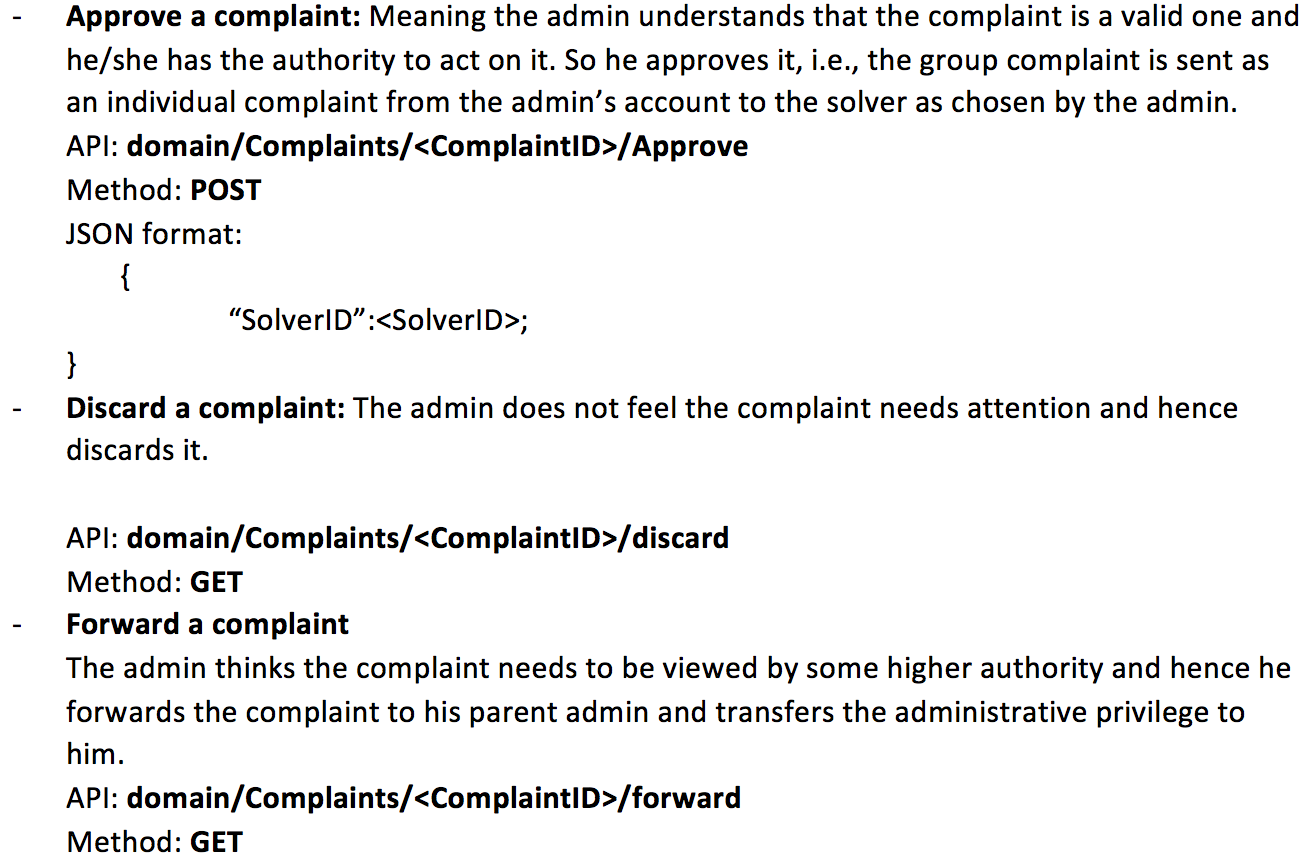
\includegraphics[scale=.5]{6.png}
            \end{minipage}
            \newline
            
\item \textbf{Polling:} This includes starting a poll by an administrator, choosing a choice by a user, or extending deadline by an administrator.
\begin{minipage}{\linewidth}
	       
	        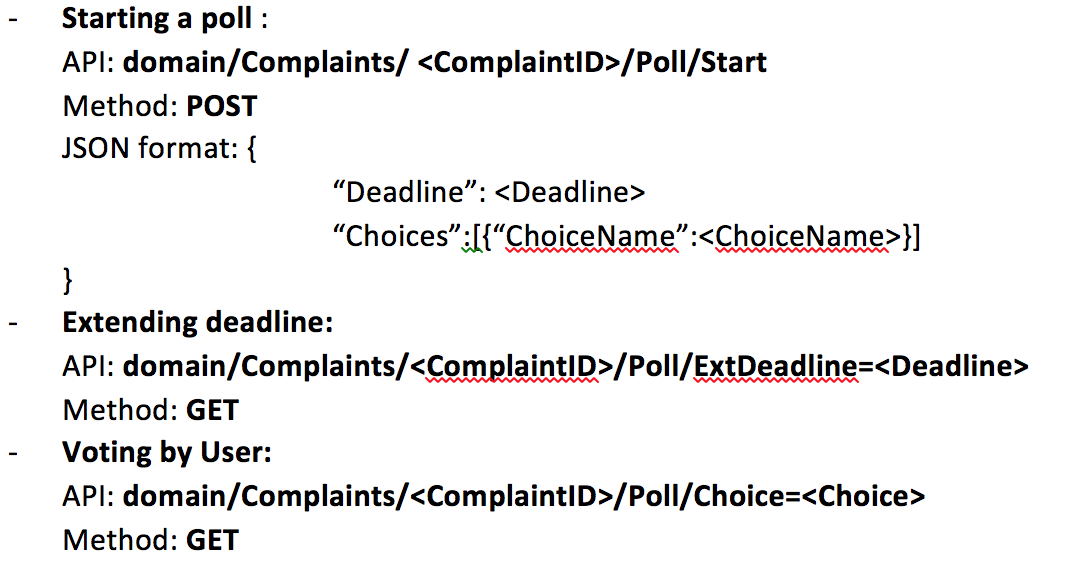
\includegraphics[scale=.5]{7.png}
            \end{minipage}
            \newline
\item \textbf{Viewing a particular complaint:} Previously, we have defined APIs to view all complaints of a particular category. Now to see the details, the user can click on that particular complaint and modify the status if he/she is an administrator.
\newline
\begin{minipage}{\linewidth}
	       
	        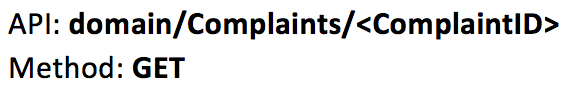
\includegraphics[scale=.5]{8.png}
            \end{minipage}
            \newline
\item \textbf{Changing the status of individual level complaints: }
We have already considered these for group level complaints. Here we will deal with individual complaint version of the group level complaints or simple individual complaints. The status is resolved or unresolved.
\newline
\begin{minipage}{\linewidth}
	       
	        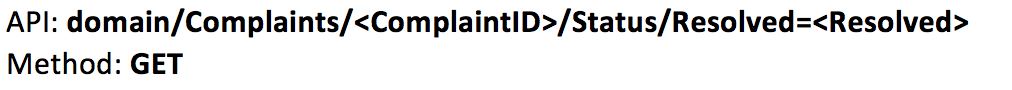
\includegraphics[scale=.5]{9.png}
            \end{minipage}
            \newline
\item \textbf{Viewing complaints by the solvers:}
The solvers can view the complaints sent to them. We require APIs for these:
\newline
\begin{minipage}{\linewidth}
	       
	        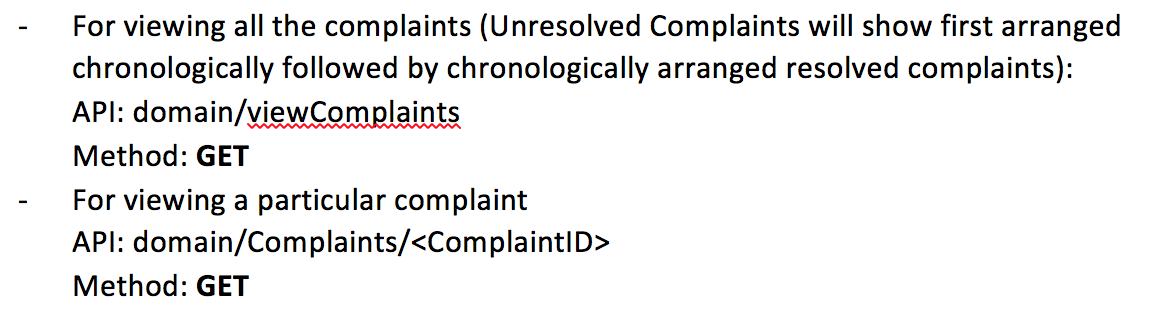
\includegraphics[scale=.5]{10.png}
            \end{minipage}
            \newline
\newpage
\section{WORK FLOW}
    \begin{minipage}{\linewidth}
	        
	        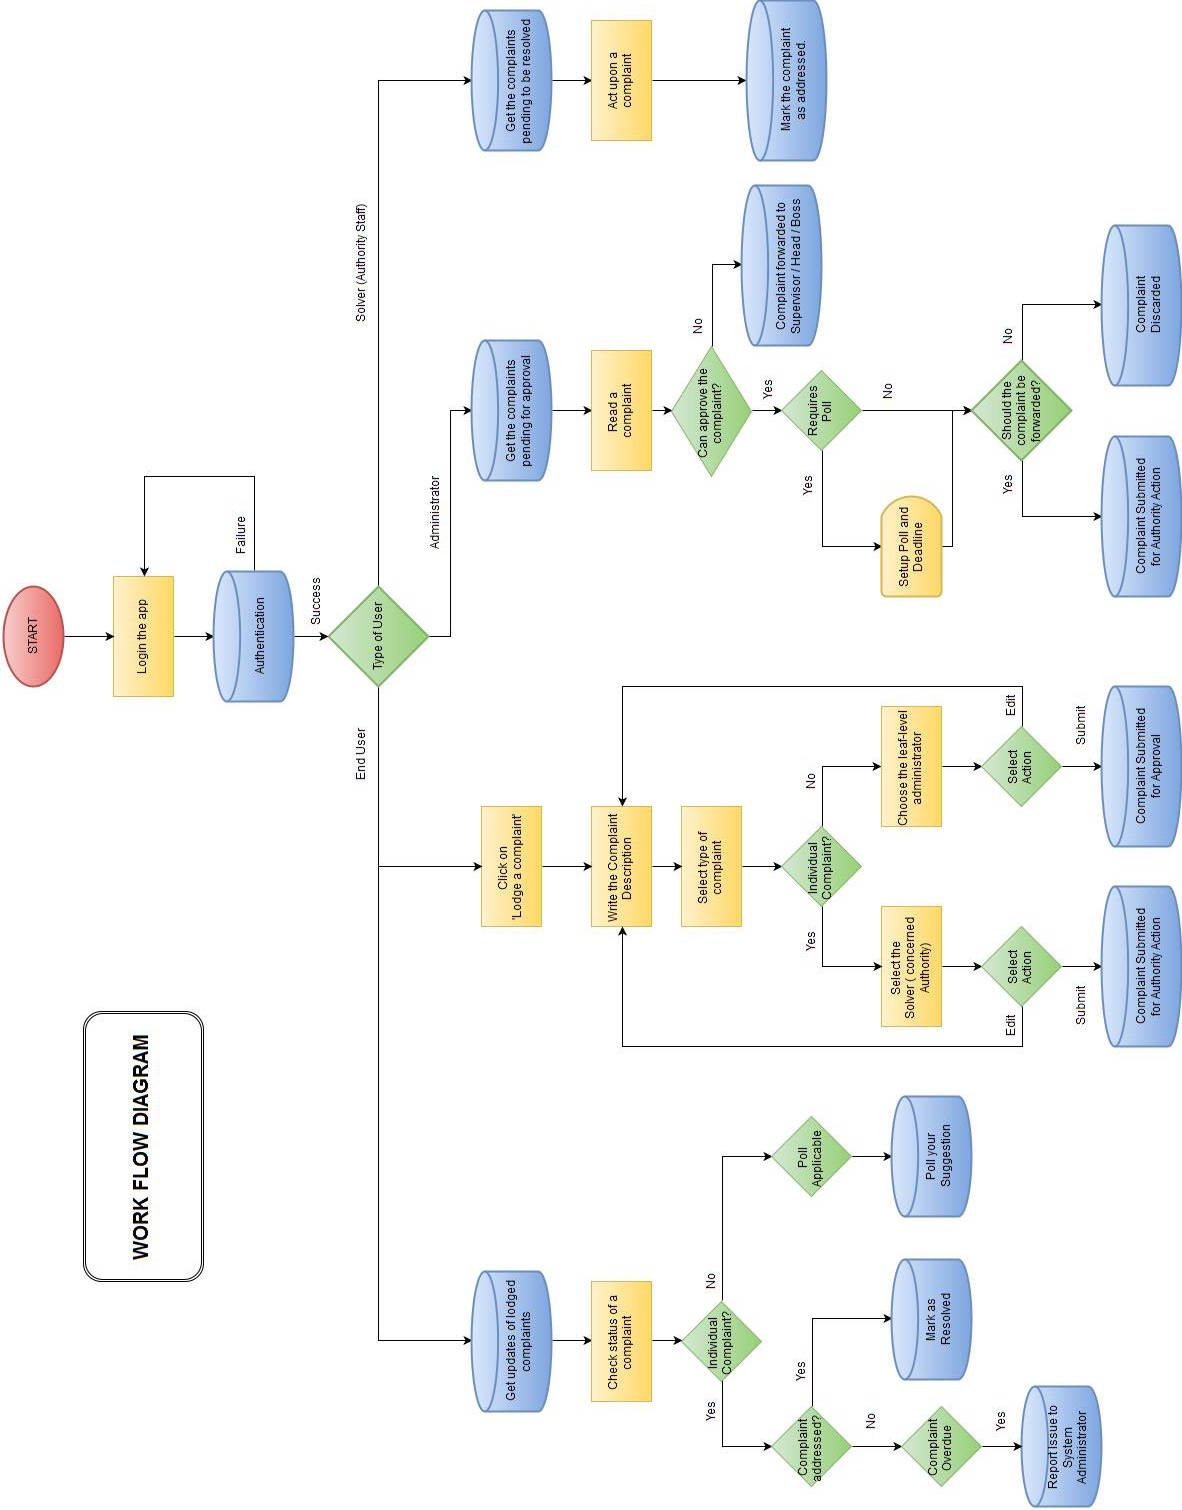
\includegraphics[scale=.3]{WorkFlow}
	        \captionof{figure}{WORK FLOW}
            \end{minipage}
            \newline
\newpage
\section{MODULARITY}
\begin{enumerate}
    \item In this application, to store the information regarding the User and Complaint following classes need to be created :
\begin{enumerate}
    \item USER
    \item ADMIN
    \item SOLVER
    \item COMPLAINT
    \subitem INDIVIDUAL COMPLAINT
    \subitem GROUP COMPLAINT
    
    
    
\end{enumerate}
\item Complaint Viewing would require:
\begin{enumerate}
    \item Linked Lists of type Complaint
    \item Complaint Layout Class which gives the display for one complaint. For each complaint in the linked list, an object of type complaint layout must be defined dynamically so that the app is able to display all the complaints.
    
    
    
    
\end{enumerate}

\end{enumerate} 
\newpage
\section{INTERFACE}
\newline
\newline

            \begin{minipage}{\linewidth}
	        \centering
	        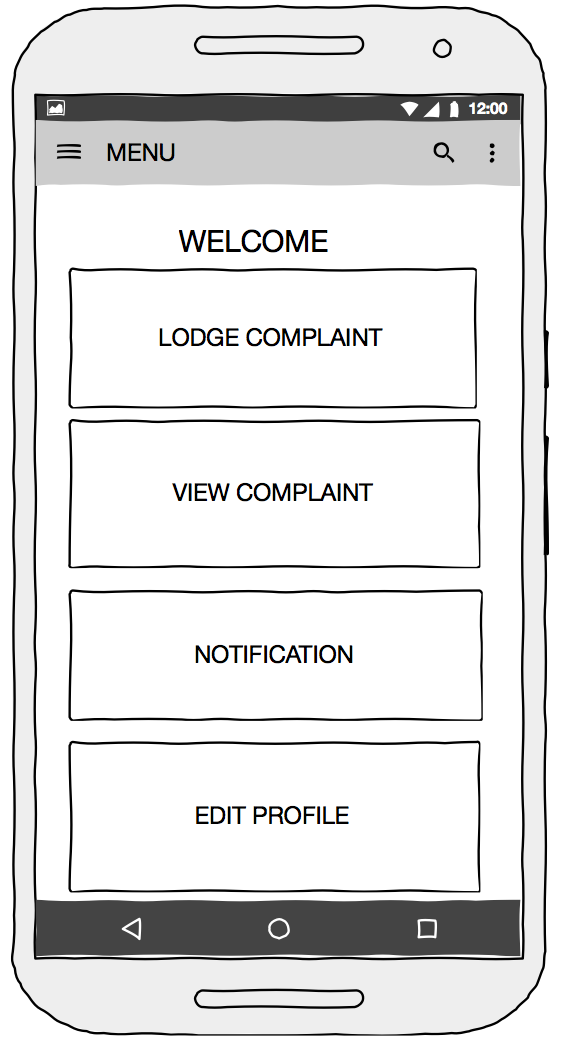
\includegraphics[scale=.8]{WELCOME_1.png}
	        \captionof{figure}{WELCOME PAGE}
            \end{minipage}
            \newpage
            \begin{minipage}{\linewidth}
	        \centering
	        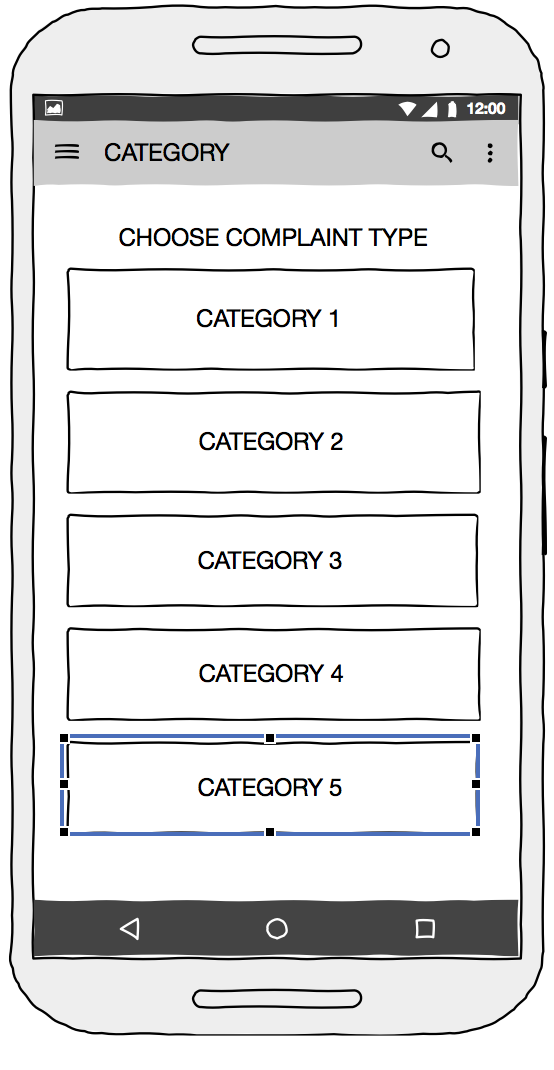
\includegraphics[scale=.8]{category1.png}
	        \captionof{figure}{CATEGORY}
            \end{minipage}
            \newpage
            \begin{minipage}{\linewidth}
	        \centering
	        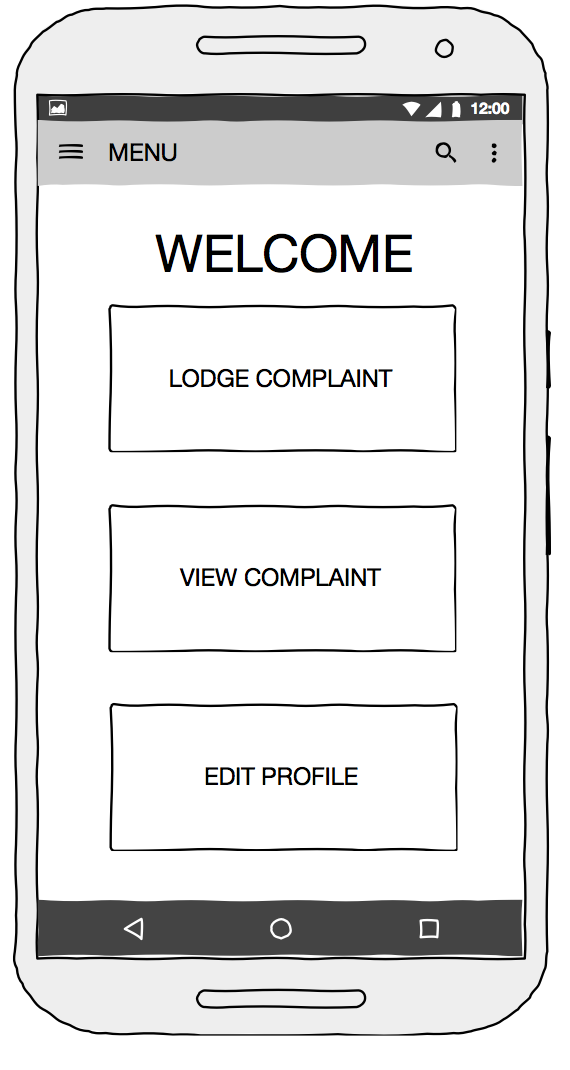
\includegraphics[scale=.8]{WELCOME1.png}
	        \captionof{figure}{WELCOME PAGE}
            \end{minipage}
            \newpage
            \begin{minipage}{\linewidth}
	        \centering
	        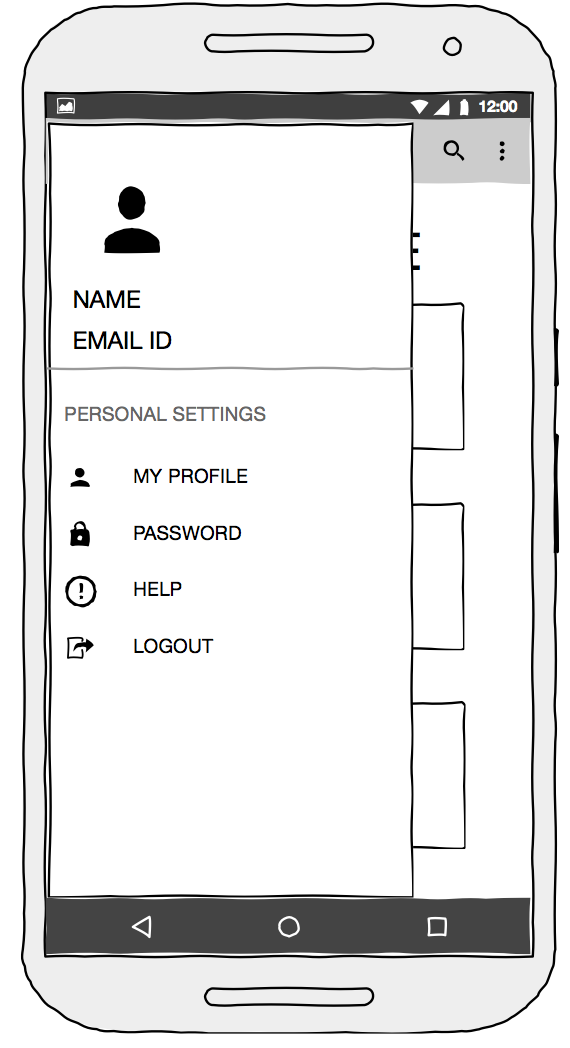
\includegraphics[scale=.8]{WELCOME2.png}
	        \captionof{figure}{WELCOME NAVIGATION BAR}
            \end{minipage}
            \newpage
            \begin{minipage}{\linewidth}
	        \centering
	        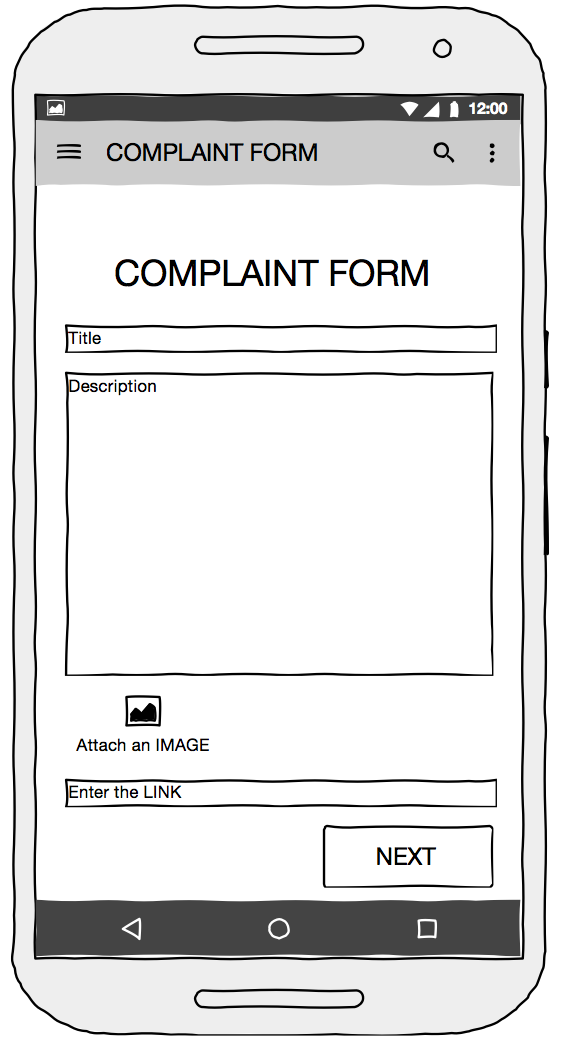
\includegraphics[scale=.8]{Complaint_Form.png}
	        \captionof{figure}{COMPLAINT FORM}
            \end{minipage}
            \newpage
            \begin{minipage}{\linewidth}
	        \centering
	        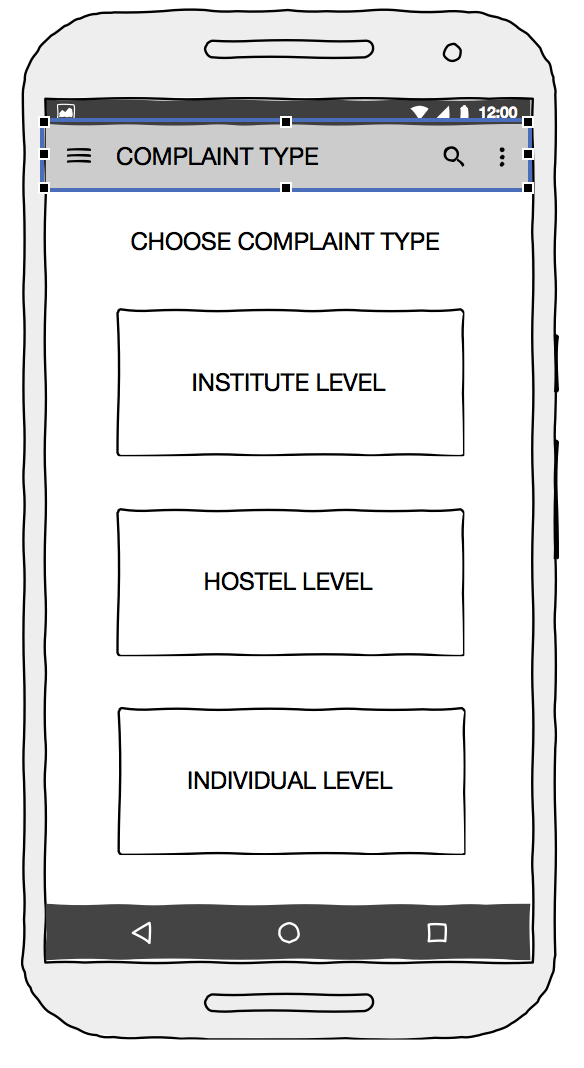
\includegraphics[scale=.8]{Complaint_Type.png}
	        \captionof{figure}{COMPLAINT TYPE}
            \end{minipage}
            \newpage
            \begin{minipage}{\linewidth}
	        \centering
	        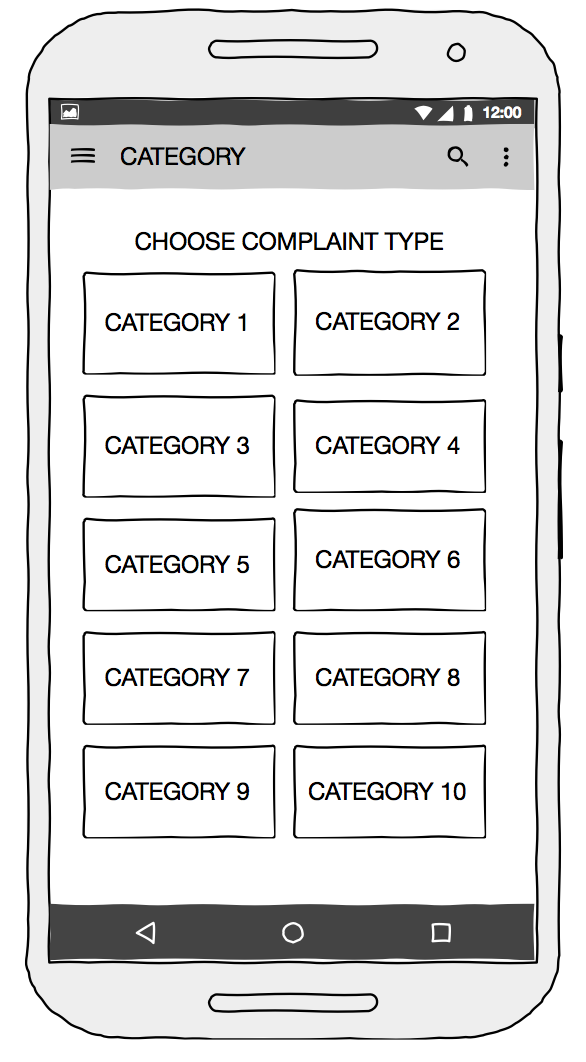
\includegraphics[scale=.8]{CATEGORY.png}
	        \captionof{figure}{CATEGORY}
            \end{minipage}
            
            


All the above screens created in WIREFRAME to show a representation of the final diagram.
\end{enumerate}
        


\end{itemize}

Report compiled by {\em Sauhard Gupta 2013ME10117}.
\newpage
\bibliography{references}\\
\textbf{\textit{REFERENCES:-}}\\
\\
http://developer.android.com \\
http://stackoverflow.com    \\
https://github.com          \\


\end{document}
